\documentclass{beamer}
\usepackage[utf8]{inputenc}

\usetheme{Madrid}
\usecolortheme{default}
\usepackage{amsmath,amssymb,amsfonts,amsthm}
\usepackage{txfonts}
\usepackage{tkz-euclide}
\usepackage{listings}
\usepackage{adjustbox}
\usepackage{array}
\usepackage{tabularx}
\usepackage{gvv}
\usepackage{lmodern}
\usepackage{circuitikz}
\usepackage{tikz}
\usepackage{graphicx}

\setbeamertemplate{page number in head/foot}[totalframenumber]

\usepackage{tcolorbox}
\tcbuselibrary{minted,breakable,xparse,skins}



\definecolor{bg}{gray}{0.95}
\DeclareTCBListing{mintedbox}{O{}m!O{}}{%
	breakable=true,
	listing engine=minted,
	listing only,
	minted language=#2,
	minted style=default,
	minted options={%
		linenos,
		gobble=0,
		breaklines=true,
		breakafter=,,
		fontsize=\small,
		numbersep=8pt,
		#1},
	boxsep=0pt,
	left skip=0pt,
	right skip=0pt,
	left=25pt,
	right=0pt,
	top=3pt,
	bottom=3pt,
	arc=5pt,
	leftrule=0pt,
	rightrule=0pt,
	bottomrule=2pt,
	toprule=2pt,
	colback=bg,
	colframe=orange!70,
	enhanced,
	overlay={%
		\begin{tcbclipinterior}
			\fill[orange!20!white] (frame.south west) rectangle ([xshift=20pt]frame.north west);
	\end{tcbclipinterior}},
	#3,
}
\lstset{
	language=C,
	basicstyle=\ttfamily\small,
	keywordstyle=\color{blue},
	stringstyle=\color{orange},
	commentstyle=\color{green!60!black},
	numbers=left,
	numberstyle=\tiny\color{gray},
	breaklines=true,
	showstringspaces=false,
}
%------------------------------------------------------------
%This block of code defines the information to appear in the
%Title page
\title %optional
{4.7.47}
%\subtitle{A short story}

\author % (optional)
{Hema Havil - EE25BTECH11050}



\begin{document}
	
	\frame{\titlepage}
	\begin{frame}{Question}
		 The foot of perpendiculars from the point (2, 3) on the line $y = 3x + 4$ is given by
         \end{frame}
\begin{frame}{Theoretical Solution}
         Let the given point be P=(2,3) and let the foot of perpendicular be Q and let the given line be written as,
         \begin{align}
             \vec{n}^T\vec{x}=c
         \end{align}
         where\\
         \begin{align*}
             \vec{n} = \myvec{3\\-1} \\ c=-4
         \end{align*}
         then Q is a point on the line, Hence it satisfies the line equation
         \begin{align}
             \vec{n}^T\vec{Q}=c
         \end{align}
         Let $\vec{m}=(a,b)$ be the direction vector of the line 
         \begin{align}
             \vec{m}^T\vec{n}=0
         \end{align}
         
\end{frame}
\begin{frame}{Theoretical Solution}
         \begin{align}
             \myvec{a\;b}\myvec{3\\-1}=0
         \end{align}
         \begin{align}
             3a=b
         \end{align}
         \begin{align}
             \vec{m}=\myvec{1\\3}
         \end{align}
         Then m is perpendicular to direction vector along PQ\\
         \begin{align}
             \vec{m}^T(\vec{Q}-\vec{P})=0
         \end{align}
         \begin{align}
             \vec{m}^T\vec{Q}=\vec{m}^T\vec{P}
         \end{align}
         from equation (0.2) and (0.8) we can write 
\end{frame}
\begin{frame}{Theoretical Solution}
    \begin{align}
             \myvec{\vec{m}\;\;\vec{n}}^T\vec{Q}=\myvec{\vec{m}^T\vec{P}\\c}
         \end{align}
         We can find the value of $\vec{m}^T\vec{P}$
         \begin{align}
             \vec{m}^T\vec{P}=\myvec{1\;3}\myvec{2\\3}=\myvec{2+9}=\myvec{11}
         \end{align}
         From this we can find Q, substitute values in (9)
         \begin{align}
             \myvec{1\;\;\;\;3\\3\;-1}^T\vec{Q}=\myvec{11\\-4}
         \end{align}
         \begin{align}
             \myvec{1\;\;\;\;3\\3\;-1}\vec{Q}=\myvec{11\\-4}
         \end{align}
         This can be solved using augmented matrix and let the augmented matrix be A
\end{frame}
\begin{frame}{Theoretical Solution}
    \begin{align}
             \vec{A}=\myvec{1\;\;\;\;3\;\;\;\;11\\3\;-1\;-4}
         \end{align}
         $R_2\rightarrow{R_2-3R_1}$
         \begin{align}
             \vec{A}=\myvec{1\;\;\;\;3\;\;\;\;11\\0\;-10\;-37}
         \end{align}
         $R_1\rightarrow{R_1+\frac{3}{10}R_2}$ \hspace{1cm}
         $R_2\rightarrow{\frac{-1}{10}R_2}$
         \begin{align}
             \vec{A}=\myvec{1\;\;\;\;0\;\;\;\;\frac{-1}{10}\\\\0\;\;\;1\;\;\;\;\frac{-37}{10}}
         \end{align}
         Therefore from (0.15) the value of Q is
         \begin{align}
             \vec{Q}=\myvec{\frac{-1}{10}\\\\ \frac{-37}{10}}
         \end{align}
\end{frame}
	\begin{frame}[fragile]
	\frametitle{C Code- Computing the unit vector}
	
	\begin{lstlisting}
#include <stdio.h>
void solve_system(double a00, double a01,
                  double a10, double a11,
                  double b0,  double b1,
                  double *rx,   double *ry)
{
    double det = a00 * a11 - a01 * a10;
    if (det == 0.0) {
        /* Singular matrix -- not expected here */
        *rx = 0.0;
        *ry = 0.0;
        return;
    }
    *rx = (b0 * a11 - b1 * a01) / det;
    *ry = (a00 * b1 - a10 * b0) / det;
}
	\end{lstlisting}
\end{frame}

\begin{frame}[fragile]
	\frametitle{Python Code using shared output}
	\begin{lstlisting}
import ctypes
import numpy as np
import matplotlib.pyplot as plt

# Load shared library (adjust path if needed)
lib = ctypes.CDLL('./4.7.47.so')

# declare argtypes: 6 doubles for matrix and RHS, and two double* for outputs
lib.solve_system.argtypes = [
    ctypes.c_double, ctypes.c_double,
    ctypes.c_double, ctypes.c_double,
    ctypes.c_double, ctypes.c_double,
    ctypes.POINTER(ctypes.c_double), ctypes.POINTER(ctypes.c_double)
]



	\end{lstlisting}
\end{frame}
\begin{frame}[fragile]
	\frametitle{Python Code using shared output}
	\begin{lstlisting}	
# Problem data
P = np.array([2.0, 3.0])         # given point P
# Line: y = 3x + 4
# We form the 2x2 linear system derived in the method:
# [1  3] Q = [m^T P]  where m = (1,3)
# [3 -1]     [   c  ]  where c = -4 (because n = (3,-1), n^T x = c -> 3x - y = -4)
A = np.array([[1.0, 3.0],
              [3.0, -1.0]])
b = np.array([ (1.0*P[0] + 3.0*P[1]),  # m^T P = [1 3] dot P
               -4.0 ])                 # c = -4

# Prepare output doubles
rx = ctypes.c_double()
ry = ctypes.c_double()


	\end{lstlisting}
\end{frame}
\begin{frame}[fragile]
  \frametitle{Python Code using shared output}
    \begin{lstlisting}
        # Call C function
lib.solve_system(A[0,0], A[0,1],
                 A[1,0], A[1,1],
                 b[0],    b[1],
                 ctypes.byref(rx), ctypes.byref(ry))

Q = np.array([rx.value, ry.value])

print("Foot of perpendicular Q =", Q)

# Plotting
x = np.linspace(-3, 4, 400)
y_line = 3*x + 4          # the line y = 3x + 4

plt.figure(figsize=(7,6))
plt.plot(x, y_line, label='Line: y = 3x + 4', linewidth=2)


    \end{lstlisting}
\end{frame}
\begin{frame}[fragile]
  \frametitle{Python Code using shared output}
    \begin{lstlisting}
        # Plot the given point P and foot Q
plt.scatter([P[0]], [P[1]], marker='o', s=80, label='P (2,3)')
plt.scatter([Q[0]], [Q[1]], marker='o', s=80, label=f'Q ({Q[0]:.3f}, {Q[1]:.3f})', color='red')

# Draw the perpendicular segment PQ
plt.plot([P[0], Q[0]], [P[1], Q[1]], '--', linewidth=1.8, label='Perpendicular PQ')

# For visual reference, draw direction vector of the line at Q (scaled)
dir_vec = np.array([1.0, 3.0])
plt.arrow(Q[0], Q[1], 0.6*dir_vec[0], 0.6*dir_vec[1], head_width=0.12, head_length=0.18, length_includes_head=True)
    \end{lstlisting}
\end{frame}
\begin{frame}[fragile]
  \frametitle{Python Code using shared output}
    \begin{lstlisting}
       plt.gca().set_aspect('equal', adjustable='box')
plt.xlim(min(-3, P[0]-2), max(4, P[0]+2))
plt.ylim(min(-1, P[1]-2), max(6, P[1]+3))
plt.xlabel('x')
plt.ylabel('y')
plt.title('Foot of Perpendicular from P')
plt.grid(True)
plt.legend()
plt.tight_layout()
plt.show() 
    \end{lstlisting}
\end{frame}
\begin{frame}{Plot by python using shared output from c}
	\begin{center}
	\begin{figure}[H]
		\centering
		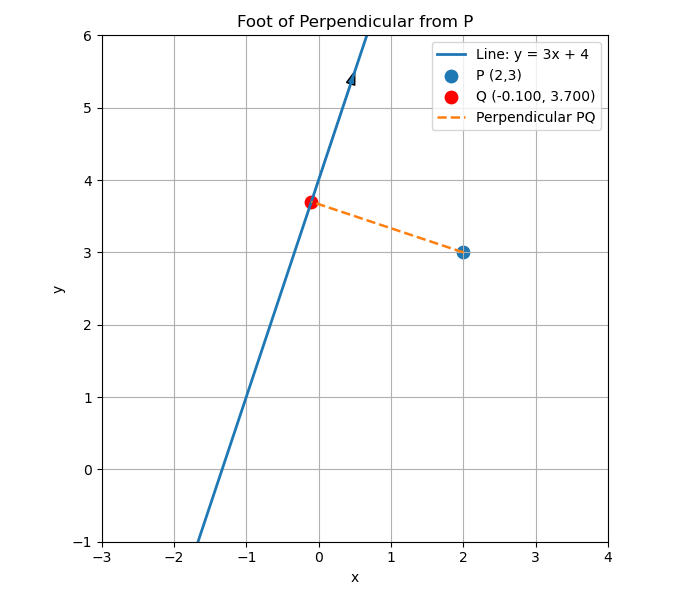
\includegraphics[width = 0.7\columnwidth]{figs/fig1.png}
		\caption{Plot of the foot of perpendicular of P}
		\label{fig1}
	\end{figure}
	\end{center}
\end{frame}
\begin{frame}[fragile]
     \frametitle{Python code for the plot}
\begin{lstlisting}
    import numpy as np
import matplotlib.pyplot as plt

# Given point P and line y = 3x + 4
P = np.array([2.0, 3.0])

# Normal vector (from line 3x - y + 4 = 0) and direction vector
n = np.array([3.0, -1.0])  # normal vector
m = np.array([1.0, 3.0])   # direction vector, since m.T n = 0
c = -4.0                   # constant term (3x - y = -4)

# Construct linear system [m^T; n^T] Q = [m^T P; c]
A = np.array([[1.0, 3.0],
              [3.0, -1.0]])
b = np.array([np.dot(m, P), c])
# Solve for Q using numpy
Q = np.linalg.solve(A, b)
print(f"Foot of perpendicular Q = ({Q[0]:.3f}, {Q[1]:.3f})")
\end{lstlisting}
\end{frame}
\begin{frame}[fragile]
   \frametitle{Python code for the plot}
    \begin{lstlisting}
# Prepare line for plotting
x = np.linspace(-3, 4, 400)
y_line = 3*x + 4  # line: y = 3x + 4

# Plot setup (same style as before)
plt.figure(figsize=(7,6))
plt.plot(x, y_line, label='Line: y = 3x + 4', linewidth=2)
# Plot points P and Q
plt.scatter(P[0], P[1], color='blue', s=80, label='P (2,3)')
plt.scatter(Q[0], Q[1], color='red', s=80, label=f'Q ({Q[0]:.2f}, {Q[1]:.2f})')
# Draw perpendicular PQ
plt.plot([P[0], Q[0]], [P[1], Q[1]], 'k--', linewidth=1.8, label='Perpendicular PQ')

 \end{lstlisting}
\end{frame}
\begin{frame}[fragile]
  \frametitle{Python code for the plot}
    \begin{lstlisting}
# Draw a small arrow showing the line direction at Q
dir_vec = m / np.linalg.norm(m)
plt.arrow(Q[0], Q[1], 0.6*dir_vec[0], 0.6*dir_vec[1],
          head_width=0.12, head_length=0.18,
          length_includes_head=True, color='green')
          # Axes formatting
plt.gca().set_aspect('equal', adjustable='box')
plt.xlim(min(-3, P[0]-2), max(4, P[0]+2))
plt.ylim(min(-1, P[1]-2), max(6, P[1]+3))
plt.xlabel('x')
plt.ylabel('y')
plt.title('Foot of Perpendicular from P')
plt.legend()
plt.grid(True)
plt.tight_layout()
plt.show()
    \end{lstlisting}
\end{frame}
 \begin{figure}
     \centering
     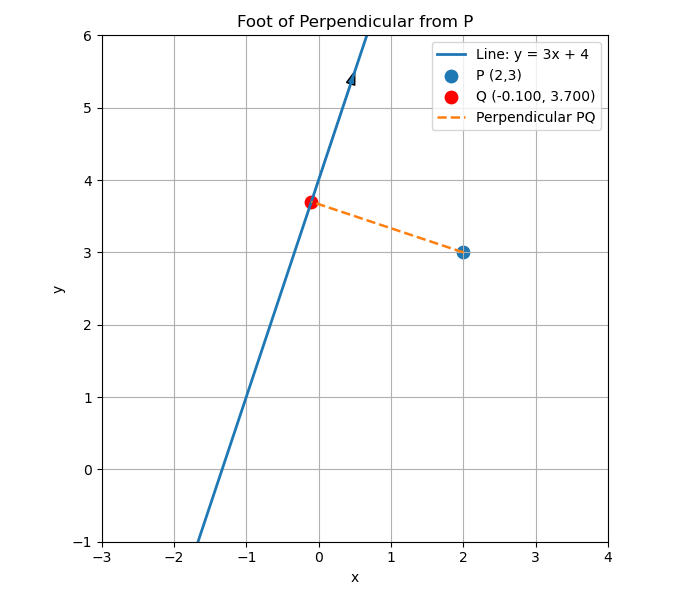
\includegraphics[width=0.7\linewidth]{figs/fig1.png}
     \caption{Plot of foot of perpendicular of point P}
     \label{fig2}
 \end{figure}
\end{document}